\chapter{Introducción}

El objetivo de este proyecto es construir un software con el que poder visualizar e interactuar con los datos DICOM obtenidos al someter a una escultura a una Tomografía Axial Computerizada (TAC o TC). 

Para ello se hará uso de VTK, que proporciona una serie de librerías en C++ para facilitar operaciones sobre datos DICOM, y de Qt, para la Interfaz Gráfica de Usuario (GUI).

Antes de empezar con el proyecto en sí, se definirán conceptos como DICOM o TC que se usarán a lo largo de éste y conviene saber lo que son, así como las distintas herramientas que se utilizarán.

\section{Obtención de datos DICOM mediante una TC}

DICOM (\textit{Digital Imaging and Comunication in Medicine}) es el estándar internacional para manejar, visualizar, almacenar, imprimir y transmitir imágenes de pruebas médicas (ISO12052) \cite{about_dicom}. 

Al contrario de lo que se puede pensar en un principio, DICOM es más que un formato de imagen, es un protocolo que abarca la transferencia, el almacenamiento y la visualización \cite{dicom_intro_and_guide}.

Pese a que su uso está mayoritariamente extendido en el campo en el que nació (la medicina) para obtener imágenes de cortes de partes del cuerpo de un paciente con fines diagnósticos, se puede usar en otros, como el de la restauración de bienes culturales, como es el caso de este proyecto.

En un archivo DICOM hay almacenado, además de metadatos, una imagen \cite{dicom_classes_vtk} (Figura \ref{fig:prostate_dicom}).

\begin{figure}[H]
	\centering
	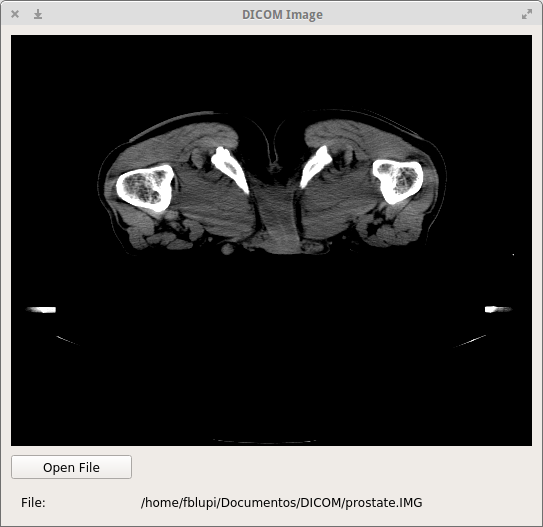
\includegraphics[width=10cm]{imagenes/prostate_dicom}
	\caption{Imagen DICOM de una próstata visualizada con un programa diseñado para visualizar archivos DICOM}
	\label{fig:prostate_dicom}
\end{figure}

\begin{figure}[H]
	\centering
	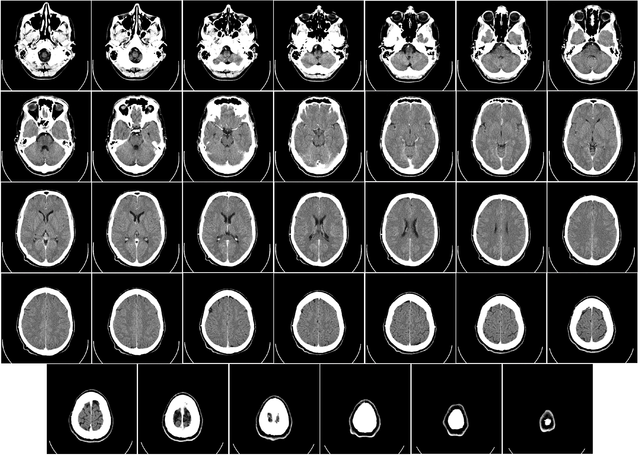
\includegraphics[width=10cm]{imagenes/brain_dicom_serie}
	\caption{Serie de imágenes DICOM extraídas de un TAC realizada a un cerebro}
	\label{fig:brain_dicom_serie}
\end{figure}

Cuando se realiza una TC se obtienen una serie de imágenes 2D (Figura \ref{fig:brain_dicom_serie}) de cortes del objeto al que se le realiza el escáner. Éstas imágenes se encapsulan en archivos DICOM, y con todas ellas se puede pasar a un espacio en 3D y llegar a construir un modelo volumétrico en el que para cada voxel (Volumetric Pixel) se tiene el valor de densidad del objeto en ese punto.

El cómo se obtienen las imágenes con una TC no es objeto de estudio de este proyecto, por lo que no se entrará en mucho detalle. En muy resumidas cuentas, el aparato emite un haz de rayos X desde distintos ángulos al objeto y unos sensores recogen la radiación que absorbe en cada una de estas emisiones. Obteniendo el resultado final del promedio de todas las mediciones que realizan los sensores \cite{tac}. 

Para renderizar la imagen con una técnica de Direct Volume Rendering (DVR) hay que darle a cada voxel un valor de color y opacidad. Esto se realizará con lo que se denomina función de transferencia (de la que se hablará exhaustivamente más adelante) que a partir de los valores de densidad y gradiente de cada voxel obtiene un valor de color y opacidad y mediante \textit{ray casting} o cualquier otra técnica de DVR se consigue el color para un pixel. Aquí es donde entrará en juego VTK, una librería que ayudará enormemente en la realización de estas tareas.

\section{VTK} 

VTK es una librería gráfica de alto nivel desarrollada por la compañía Kitware.

% Hablar un poquito más de esto

\section{Trabajos previos}

Como ya se ha comentado anteriormente, el uso de las imágenes obtenidas con las TCs está muy extendido en el campo de la medicina, aunque puede ser usado en otros. 

Ha tenido bastante repercursión en estudios anatómicos del estado actual de momias \cite{mummies} y para realizar reconstrucciones de su posible estado anterior \cite{mummies_reconstruction}.

En el caso de estudio de este proyecto, la restauración de bienes culturales, obviamente, también puede aplicarse.

Tradicionalmente, se han utilizado radiografías para examinar el estado de las esculturas, pero el uso de TCs hace que se puedan obtener resultados que permitan realizar exámenes más precisos y exhaustivos a los restauradores.

Se podría hacer uso de herramientas médicas como OsiriX \cite{osirix}, AMILab \cite{amilab} o RadiAnt; pero proporcionan presets para visualizar materiales de los que están compuestos los organismos humanos y la mayoría de ellas tienen un precio de licencia muy elevado.

También se podrían utilizar herramientas más genéricas como 3DSlicer \cite{slicer}, desarrollada por la misma compañía que VTK. No obstante, tiene muchas funcionalidades que no utilizarían los restauradores y hacen de ella una herramienta demasiado compleja.

Incluso podrían hacer uso de software específico para la visualización de esculturas, aunque hay muy pocas herramientas que tengan funcionalidad para trabajar con conjuntos de datos volumétricos. La más referenciada es Hyper3D \cite{hyper3D} pero los resultados obtenidos no son buenos \ref{fig:hyper3d_results}.

\begin{figure}[H]
	\centering
	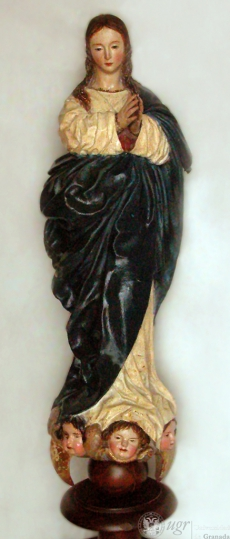
\includegraphics[height=12cm]{imagenes/inmaculada_concepcion_real}
	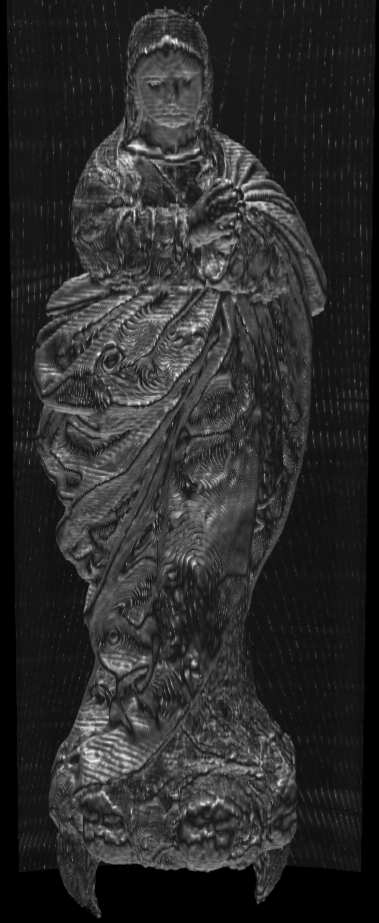
\includegraphics[height=12cm]{imagenes/inmaculada_concepcion_hyper3d}
	\caption{A la izquierda escultura de la Inmaculada Concepción. A la derecha su reconstrucción volumétrica usando Hyper3D y su preset para madera}
	\label{fig:hyper3d_results}
\end{figure}

\section{Motivación}

El resultado insatisfactorio obtenido con las herramientas disponibles ha motivado la idea de desarrollar \myTitle, un software creado para que los restauradores puedan examinar esculturas de madera policromadas y así conocer los materiales de los que están compuestas, su estructura interna, observar si está dañada o ver cuántos años tiene la madera utilizada gracias a sus anillos.

Incluyendo también una serie de presets para poder visualizar unos u otros materiales sin que el usuario tenga por qué conocer los valores de densidad de estos para crear una función de transferencia que los visualice, pero proporcionando también un editor de funciones de transferencias con el que los usuarios más avezados puedan crear sus propios presets y exportarlos para que puedan ser utilizados por los demás.
